\documentclass[10pt]{article}

\usepackage[utf8]{inputenc}
\usepackage[T1]{fontenc}
\usepackage[polish]{babel}
\usepackage{listings}
\usepackage{xcolor}
\usepackage{amsmath, amssymb, amsthm}
\usepackage{graphicx}
\usepackage{geometry}
\usepackage{hyperref}
\usepackage{fancyhdr}
\usepackage{enumitem}
\usepackage{titlesec}

\geometry{
    a4paper,
    left=25mm,
    right=25mm,
    top=25mm,
    bottom=25mm
}

\pagestyle{fancy}
\fancyhf{}
\fancyhead[L]{PW}
\fancyhead[R]{\thepage}
\fancyfoot[C]{}

\newtheorem{theorem}{Theorem}[section]
\newtheorem{lemma}[theorem]{Lemma}
\newtheorem{corollary}[theorem]{Corollary}
\newtheorem{definition}[theorem]{Definition}
\newtheorem{proposition}[theorem]{Proposition}
\newtheorem{remark}[theorem]{Remark}

\newcommand{\R}{\mathbb{R}}
\newcommand{\C}{\mathbb{C}}
\newcommand{\N}{\mathbb{N}}
\newcommand{\Z}{\mathbb{Z}}
\newcommand{\Q}{\mathbb{Q}}
\newcommand{\eps}{\varepsilon}
\newcommand{\norm}[1]{\left\lVert#1\right\rVert}
\newcommand{\abs}[1]{\left|#1\right|}

\titleformat{\section}{\normalfont\Large\bfseries}{\thesection}{1em}{}
\titleformat{\subsection}{\normalfont\large\bfseries}{\thesubsection}{1em}{}
\titleformat{\subsubsection}{\normalfont\normalsize\bfseries}{\thesubsubsection}{1em}{}

% Styl listingów.
\lstset{basicstyle=\footnotesize\ttfamily,breaklines=true}
\lstset{framextopmargin=50pt,frame=bottomline}

\title{Przetwarzanie dokumentów tekstowych.}
\author{Łukasz Ambroziak, Adam Kordeczka}

\begin{document}

\maketitle

\begin{abstract}
  Praca zaliczeniowa przedmiotu: Projektowanie rozwiązań Big Data na kierunku: Big Data - przetwarzanie i analiza dużych zbiorów danych organiozwanych przez Politechnikę Warszawską. Celem pracy było stworzenie skalowalnego, rozproszonego systemu umożliwiającego: (i) wykonywanie analiz ad-hoc z wykorzystaniem MongoDB, (ii) przetwarzenie danych wsadowych z wykorzystaniem Apache Spark, (iii) aplikowanie współczesnych metod przetwarzania języka naturalnego do danych o typie tekstowym, (iv) przygotowanie metod przeszukiwania dużego wolumenu danych tekstowych, które zasilą system Retrieval Augmented Generation (dalej: RAG). Część prezentacyjną uzupełnia interfejs graficzny umożliwiający komunikację z modelami uczenia maszynowego: DistilBERT oraz Phi-3.
\end{abstract}

\section{Wprowadzenie}

Motywacją dla przygotowania szytego na miarę systemu RAG było:

\begin{itemize}
  \item ocena możliwości stosowania systemów RAG jako alternatywy dla fine-tuningu dużych modeli językowych w rozwiązywaniu konkretnych problemów (często wymagających specjalistycznej wiedzy domenowej), np. przeszukiwania aktów prawnych, publikacji naukowych z dziedziny fizyki, itp.,
  \item przygotowanie modułowego, elastycznego i skalowalnego systemu umożliwiającego niskokosztowe dostosowywanie do konkretnych zadań - specjalizacja zamiast generalizacji,
  \item uniknięcie integracji z API dużych modeli językowych; założeniem było badanie możliwości stosowania mniejszych modeli językowych, które mogą być wdrażane w środowiskach on-premise bez dostępu do dużych zasobów obliczeniowych a jednocześnie gwarantując prywatność przetwarzanych danych.
\end{itemize}

Stosowanie systemów RAG jako alternatywy dla fine-tuningu dużych modeli językowuch stanowi obiecujący sposób na wdrażanie nowoczesnych systemów przetwarzania języka naturalnego w organizacjach nie posiadających dostępu do dużych zasobów obliczeniowych, co w szczególności dotyczy sytuacji: niewystarczających środków finansowych lub braku kompetencji w dostrajaniu dużych modeli językowych do rozwiązywania zadań wewnątrz organizacji. Meta inwestuje 30 miliardów dolarów\footnote{\url{https://fusionchat.ai/news/metas-strategic-move-30-billion-investment-in-nvidia-gpus}} w zakup kart graficznych wykorzystywanych do budowy modeli uczenia maszynowego. Stanowi to 4.35\% polskiego Produktu Krajowego Brutto\footnote{\url{https://tradingeconomics.com/poland/gdp}} a więc więcej niż sumaryczne wydatki na obronność kraju jako członka NATO. Oczywistym wydaje się zatem, że utrzymanie konkurencyjności polskiej gospodarki w zakresie stosowania nowoczesnych metod uczenia maszynowego wymaga alternatywnej drogi w wyścigu z gigantami technologicznymi i wzroście produktywności przez stosowanie modeli uczenia maszynowego w szerokiej skali w całej gospodarce.

Zapewnienie modułowości motywowane jest przez dostosowywanie systemu do zastanego stosu technologicznego (w tym: kompetencji pracowników). W ramach projektu przygotowano rozwiązanie oparte o ugruntowane technologie (z pominięciem specjalizowanych frameworków), co może przyspieszyć ich adopcję w organizacjach. Jednocześnie w projekcie przedstawione zostaną propozycje w jaki sposób ludzka inteligencja może wspierać systemu uczenia maszynowego we wskazywaniu obszarów, w których modele powinny poszukiwać odpowiedzi na zadane pytania.

Uniknięcie integracji z API dużych modeli językowych gwarantuje wysoką prywatność przetwarzanych danych. Współcześnie dane posiadane przez organizację stają się jej przewagą konkurencyjną. Udostępnienie tych danych, przez API, do wzbogacania dużych modeli językowych budowanych przez firmy zewnętrzne może finalnie ją zniwelować.

\section{Zbiór danych}

Zbiór danych wykorzystany w projekcie to dane pochodzące z ArXiv\footnote{Od prawie 30 lat ArXiv służy zarówno społeczeństwu, jak i społecznościom naukowym, zapewniając otwarty dostęp do artykułów naukowych z różnych dziedzin, od rozległych obszarów fizyki po liczne subdyscypliny informatyki, a także wiele innych, w tym matematykę, statystykę, inżynierię elektryczną, biologię ilościową i ekonomię. Dostęp: \url{https://www.kaggle.com/Cornell-University/arxiv})}. Z uwagi na to, że oryginalny zbiór danych jest relatywnie duży (1.1 TB i rośnie) ograniczono się do wykorzystania pliku z metadanymi w formacie json (4.1 Gb). Plik ten zawiera wpis dla każdej pracy, zawierający:

\begin{itemize}
    \item \textbf{id}: Identyfikator ArXiv (może być użyty do uzyskania dostępu do pracy, patrz poniżej)
    \item \textbf{submitter}: Osoba, która zgłosiła pracę
    \item \textbf{authors}: Autorzy pracy
    \item \textbf{title}: Tytuł pracy
    \item \textbf{comments}: Dodatkowe informacje, takie jak liczba stron i rysunków
    \item \textbf{journal-ref}: Informacje o czasopiśmie, w którym praca została opublikowana
    \item \textbf{doi}: \href{https://www.doi.org}{Cyfrowy Identyfikator Obiektu (DOI)}
    \item \textbf{abstract}: Streszczenie pracy
    \item \textbf{categories}: Kategorie / tagi w systemie ArXiv
    \item \textbf{versions}: Historia wersji
\end{itemize}

Poniżej przedstawiono strukturę przykładowego dokumentu (ze zrandomizowanymi danymi):
\begin{lstlisting}
    {
        "root": {
            "id": "0704.0001",
            "submitter": "Jan Kowalski",
            "authors": "J. Kowalski",
            "title": "Hello, world!",
            "comments": "37 pages, 15 figures; published version",
            "journal-ref": "Phys.Rev.D76:013009,2007",
            "doi": "10.1103/PhysRevD.76.013009",
            "report-no": "ANL-HEP-PR-07-12",
            "categories": "hep-ph",
            "license": "MIT",
            "abstract": "Hello, world!",
            "versions": [0: {
              "version": "v1",
              "created": "Mon, 2 Apr 2007 19:18:42 GMT"
            }],
            "update_date": "2024-05-25",
            "authors_parsed": [0: [0: "J.", 1: "Kowalski"]]
        }
    }
\end{lstlisting}

\section{Architektura}

Rysunek \ref{fig:architecture} przedstawia architekturę systemu. System składa się z czterech głównych komponentów: (i) jeziora danych (ang. data lake), w którym dane przechowywane są w formie surowej, (ii) transformwacji i ładowania danych z wykorzystaniem Apache Spark, (iii) przechowywania przetworzonych danych w bazie danych MongoDB, (iv) części prezentacyjnej, w której użytkownik może przeszukiwać dane oraz korzystać z modeli uczenia maszynowego.

\begin{figure}[h]
    \centering
    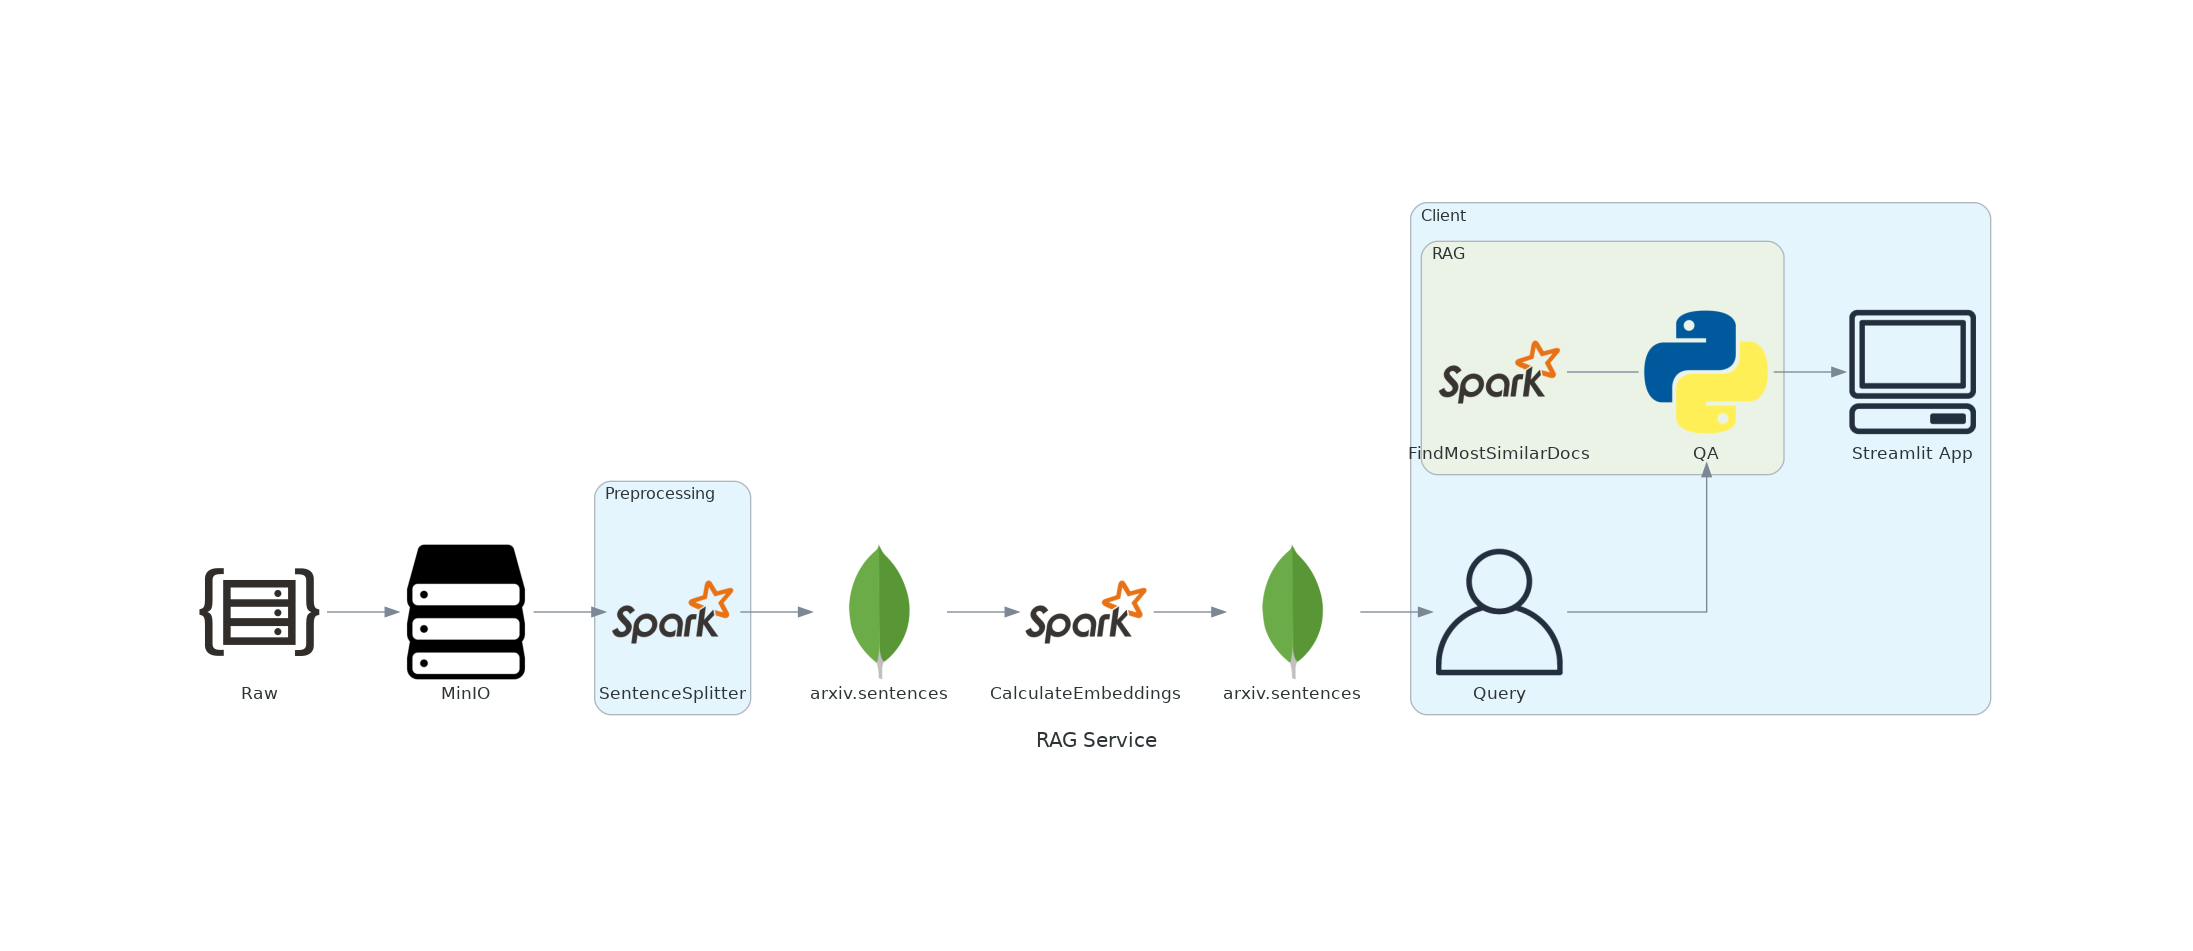
\includegraphics[width=1.0\textwidth]{images/architecture.png}
    \caption{Architektura systemu.}
    \label{fig:architecture}
\end{figure}


Infrastrukturę dofiniuje plik \texttt{docker-compose.yml}, który uruchamia kontenery z Apache Spark, MongoDB, MinIO, Jupyter. Plik załączono w \ref{s:docker-compose.yml}.

Interakcja z systemem odbywa się za pomocą pakietu Python o nazwie \texttt{rag}, który został zaimplementowany na potrzeby projektu. Pakiet posiada command-line interface implementujący następujące funkcjonalności:

\begin{lstlisting}
    # rag --help
    Usage: rag [OPTIONS] COMMAND [ARGS]...
    
    Options:
      --help  Show this message and exit.
    
    Commands:
      embeddings         Calculate embeddings.
      minio              Populate Minio with data.
      most-similar-docs  Get most similar documents.
      preprocessing      Preprocess data.
      qa                 Question & Answers.
\end{lstlisting}

\subsection{Jezioro danych}

\subsubsection{Inicjalne zasilenie danych}

Rozpoczynamy od zasilenia systemu danymi. W tym celu korzystamy z polecenia \texttt{minio} w CLI pakietu \texttt{rag}:
\begin{lstlisting}
  Usage: rag minio [OPTIONS]

  Populate Minio with data.

  Args:
    path_to_raw_data (str): The path to the raw data.
    bucket (str): The name of the Minio bucket.
    processes (int): The number of processes to use for populating Minio.
    path_to_env (str): The path to the environment file.

  Returns: The result of the `main` function from 
    `rag.datasets.populate_minio`.

Options:
  --path-to-raw-data TEXT  [required]
  --bucket TEXT            [required]
  --processes INTEGER      [required]
  --path-to-env TEXT       [required]
  --help                   Show this message and exit.
\end{lstlisting}

Implementacja polecenia jest dostępna w repozytorium projektu w ścieżce \texttt{src\/rag\/datasets\/populate\_minio.py}.

\subsubsection{Przechowywanie}

Surowe dane przechowywane są w bucket \texttt{papers} w MinIO. Każdy dokument zapisany jest w formacie JSON. Nazwą pliku jest identyfikator ArXiv. Otwiera to możliwość do późniejszego rozszerzenia plików JSON o pełną treść publikacji, np. w polu: \texttt{fulltext}.

\subsection{Transformacja i ładowanie danych}

Następnie przetwarzamy dane, aby umożliwić wykorzystanie modeli uczenia maszynowego. W tym celu korzystamy z Apache Spark. Implementacja przetwarzania danych dostępna jest w repozytorium projektu w ścieżce \texttt{src\\/rag\/processor\/preprocessing.py}. Korzystamy z polecenia \texttt{preprocessing} w CLI pakietu \texttt{rag}:

\begin{lstlisting}
  Usage: rag preprocessing [OPTIONS]

  Preprocess data.

  This function performs data preprocessing using the specified data and
  environment paths.

  Args:
    path_to_data (str): The path to the data.
    path_to_env (str): The path to the environment.

  Returns: 
    The result of the preprocessing.

Options:
  --path-to-data TEXT  [required]
  --path-to-env TEXT   [required]
  --help               Show this message and exit.
\end{lstlisting}

\subsection{Przechowywanie przetworzonych danych}

\subsection{Reprezentacje wektorowe}

Następnie, przygotowujemy reprezentację wektorowe pojedynczych zdań składających się na pełną treść abstraktów. W tym celu korzystamy z Apache Spark oraz modelu pobranego z Hugging Face. Implementacja obliczania reprezentacji wektorowych dostępna jest w repozytorium projektu w ścieżce \texttt{src\/rag\/processor\/embeddings.py}. Korzystamy z polecenia \texttt{embeddings} w CLI pakietu \texttt{rag}:

\begin{lstlisting}
  Usage: rag embeddings [OPTIONS]

  Calculate embeddings.

  This function calculates embeddings using the specified model.

  Args:
    path_to_env (str): The path to the environment.
    model (str): The name of the model to use.

  Returns: 
    The result of the `main` function from the `embeddings` module.

Options:
  --model TEXT        [required]
  --source TEXT       [required]
  --path-to-env TEXT  [required]
  --help              Show this message and exit.
\end{lstlisting}

\subsection{Część prezentacyjna}

\subsubsection{Stosowane modele}

\subsubsection{Wady i zalety stosowanych modeli}

\subsubsection{Demonstracja działania}

\section{Załączniki}
\subsection{docker-compose.yml}
\label{s:docker-compose.yml}

\begin{lstlisting}
  version: '3.8'

  services:
  
    mongo:
      image: mongo:latest
      container_name: mongodb
      ports:
        - "27017:27017"
      volumes:
        - ./data/mongo:/data/db
  
    spark:
      image: custom-spark:3.5.0
      build:
        context: .
        dockerfile: ./dockerfiles/spark
      container_name: spark
      environment:
        - SPARK_MODE=master
        - SPARK_MASTER_HOST=spark
        - SPARK_MASTER_PORT=7077
        - SPARK_RPC_AUTHENTICATION_ENABLED=no
        - SPARK_RPC_ENCRYPTION_ENABLED=no
        - SPARK_LOCAL_STORAGE_ENCRYPTION_ENABLED=no
        - SPARK_SSL_ENABLED=no
        - XDG_CACHE_HOME=/opt/bitnami/spark/.cache
      ports:
        - "8080:8080"
        - "7077:7077"
  
    spark-worker:
      image: custom-spark:3.5.0
      build:
        context: .
        dockerfile: ./dockerfiles/spark
      container_name: spark-worker
      environment:
        - SPARK_MODE=worker
        - SPARK_MASTER_URL=spark://spark:7077
        - SPARK_RPC_AUTHENTICATION_ENABLED=no
        - SPARK_RPC_ENCRYPTION_ENABLED=no
        - SPARK_LOCAL_STORAGE_ENCRYPTION_ENABLED=no
        - SPARK_SSL_ENABLED=no
        - XDG_CACHE_HOME=/opt/bitnami/spark/.cache
      depends_on:
        - spark
  
    minio:
      image: minio/minio
      ports:
        - 9000:9000
        - 9001:9001
      environment:
        - MINIO_ROOT_USER=minio
        - MINIO_ROOT_PASSWORD=miniominio
      container_name: minio
      command: server /data/minio --console-address ":9001"
      healthcheck:
        test:
          [
            "CMD",
            "curl",
            "-f",
            "http://localhost:9000/minio/health/live"
          ]
        interval: 30s
        timeout: 20s
        retries: 3
      volumes:
        - ./data/minio:/data/minio
  
    jupyter:
      image: jupyter:1.0.0
      container_name: jupyter
      build:
        context: .
        dockerfile: ./dockerfiles/jupyter
      ports:
        - "8888:8888"
        - "8501:8501" #streamlit app port
      command:
        [
          "jupyter",
          "lab",
          "--ip=0.0.0.0",
          "--port=8888",
          "--no-browser",
          "--allow-root",
          "--NotebookApp.token=''"
        ]
      volumes:
        - ./:/rag/
      depends_on:
        - mongo
        - spark
        - spark-worker
        - minio
  
  volumes:
    mongo-data:
    minio-data:
  
\end{lstlisting}

\end{document}
